\documentclass{article}
\usepackage[utf8]{inputenc}
\usepackage{amsmath}
\usepackage{amsfonts}
\usepackage{amssymb}
\usepackage{graphicx}
\usepackage[bookmarks=false]{hyperref}
\usepackage{algorithm}
\usepackage{algpseudocode}
\usepackage{booktabs}
\usepackage{multirow}

\title{STU-PID: Steering Token Usage via PID Controller for Efficient Large Language Model Reasoning}

\author{Aryasomayajula Ram Bharadwaj}
\date{}

\begin{document}

\maketitle

\begin{abstract}
Large Language Models (LLMs) employing extended chain-of-thought (CoT) reasoning often suffer from the "overthinking phenomenon," generating excessive and redundant reasoning steps that increase computational costs while potentially degrading performance. While recent work has explored static steering approaches to mitigate this issue, they lack the adaptability to dynamically adjust intervention strength based on real-time reasoning quality. We propose STU-PID (Steering Token Usage via PID controller), a novel training-free method that employs a PID controller to dynamically modulate activation steering strength during inference. Our approach combines a chunk-level classifier for detecting redundant reasoning patterns with a PID control mechanism that adaptively adjusts steering intensity based on the predicted redundancy probability. Experimental evaluation on GSM8K demonstrates that STU-PID achieves a 6\% improvement in accuracy while reducing token usage by 32\%, outperforming static steering baselines. Our method provides a principled framework for dynamic reasoning calibration that maintains reasoning quality while significantly improving computational efficiency.
\end{abstract}

\section{Introduction}

Recent advances in Large Language Models (LLMs) have demonstrated remarkable capabilities in complex reasoning tasks through extended chain-of-thought (CoT) reasoning processes \cite{wei2022chain}. Notable examples include OpenAI's o1-series models and their open-source counterparts like DeepSeek-R1 \cite{guo2025deepseek}. However, these models often suffer from the "overthinking phenomenon" \cite{sui2025stop}, where they generate excessively verbose and redundant reasoning sequences, leading to increased computational costs and potential performance degradation.

The inefficiency of current reasoning models stems from their tendency to produce unnecessary reflection and transition thoughts that divert attention from productive reasoning paths \cite{chen2025seal}. While recent work has explored various approaches to address this issue, including reinforcement learning with length rewards and supervised fine-tuning with variable-length CoT data \cite{sui2025stop}, most existing methods require expensive retraining or lack the ability to adapt dynamically during inference.

Static activation steering approaches, such as SEAL \cite{chen2025seal}, have shown promise in calibrating reasoning processes by reducing redundant thoughts through fixed steering vectors. However, these methods apply constant steering strength regardless of the dynamic nature of reasoning quality, potentially over-steering in some contexts while under-steering in others.

To address these limitations, we propose STU-PID (Steering Token Usage via PID controller), a training-free method that dynamically adjusts steering strength using a Proportional-Integral-Derivative (PID) controller. Our key contributions are:

\begin{itemize}
\item We introduce a novel adaptive steering framework that uses PID control to dynamically adjust intervention strength based on real-time reasoning quality assessment.
\item We develop a chunk-level classifier for detecting redundant reasoning patterns that serves as the feedback signal for the PID controller.
\item We demonstrate significant improvements on GSM8K, achieving 5.7\% higher accuracy with 32\% reduction in token usage compared to baseline models.
\item We provide a principled approach for dynamic reasoning calibration that maintains the benefits of activation steering while avoiding the pitfalls of static intervention.
\end{itemize}

\section{Related Work}

\subsection{Efficient Reasoning in Large Language Models}

The challenge of improving reasoning efficiency in LLMs has been extensively studied. Sui et al. \cite{sui2025stop} provide a comprehensive survey categorizing approaches into model-based, reasoning output-based, and input prompts-based methods. Model-based approaches include reinforcement learning with length rewards and supervised fine-tuning with variable-length CoT data. Reasoning output-based methods focus on compressing reasoning steps into latent representations or implementing dynamic reasoning paradigms during inference.

\subsection{Activation Steering for Reasoning Control}

Recent work has explored using activation steering to control model behavior. Chen et al. \cite{chen2025seal} propose SEAL, which categorizes reasoning into execution, reflection, and transition thoughts, then applies static steering vectors to reduce redundant reflection and transition thoughts. While effective, this approach lacks adaptability to varying reasoning contexts and may apply inappropriate steering strength across different problem complexities.

\subsection{Control Theory in Machine Learning}

PID controllers have been successfully applied in various machine learning contexts for adaptive control. Our work is the first to apply PID control principles to activation steering for reasoning calibration, providing a principled framework for dynamic intervention strength adjustment.

\section{Methodology}

\subsection{Problem Formulation}

Given a language model $M$ and an input question $q$, the model generates a response through an autoregressive process. At each step $t$, the model produces hidden representations $h_t$ that can be intervened using a control vector $v$ with strength $\alpha_t$:

$$h'_t = h_t + \alpha_t \cdot v$$

The challenge is to determine the optimal $\alpha_t$ dynamically based on the current reasoning state to minimize redundant token generation while maintaining or improving accuracy.

\subsection{STU-PID Framework}

Our STU-PID framework consists of three main components:

\subsubsection{Redundancy Classifier}

We train a lightweight classifier $C$ to detect redundant reasoning patterns at the chunk level. Given a sequence of tokens forming a reasoning chunk, the classifier outputs a probability $p_{red} \in [0,1]$ indicating the likelihood that the chunk represents redundant reasoning.

The classifier operates on chunk-level hidden representations extracted from layer $l$ of the model:
$$p_{red} = C(h_l^{chunk})$$

where $h_l^{chunk}$ represents the mean-pooled hidden states of tokens within a reasoning chunk at layer $l$.

\subsubsection{PID Controller}

The core innovation of STU-PID is the use of a PID controller to dynamically adjust steering strength. The controller maintains three components:

\begin{align}
e_t &= p_{red,t} - p_{target} \\
P_t &= K_P \cdot e_t \\
I_t &= K_I \cdot \sum_{i=0}^{t} e_i \\
D_t &= K_D \cdot (e_t - e_{t-1})
\end{align}

where $p_{target}$ is the desired redundancy probability, and $K_P$, $K_I$, $K_D$ are the proportional, integral, and derivative gains, respectively.

The steering strength is computed as:
$$\alpha_t = \max(0, \min(\alpha_{max}, \alpha_{t-1} + P_t + I_t + D_t))$$

\subsubsection{Control Vector Application}

Following previous work \cite{chen2025seal}, we construct a control vector $v$ by computing the difference between mean hidden representations of required and redundant reasoning patterns:
$$v = \mathbb{E}[h_{required}] - \mathbb{E}[h_{redundant}]$$

This vector is applied during generation when the PID controller determines intervention is necessary.

\subsection{Training and Inference}

\subsubsection{Offline Training Phase}

1. **Data Collection**: Collect a small dataset of labeled reasoning examples, categorizing reasoning chunks as "required" or "redundant."

2. **Classifier Training**: Train the redundancy classifier using chunk-level features extracted from the model's hidden states.

3. **Control Vector Extraction**: Compute the control vector from the difference in mean representations between required and redundant reasoning patterns.

4. **Hyperparameter Optimization**: Optimize PID controller parameters $(K_P, K_I, K_D)$ and target redundancy probability $p_{target}$ using a small validation set.

\subsubsection{Online Inference Phase}

During inference, STU-PID operates as follows:

\begin{figure}[h]
\centering
\begin{minipage}{\textwidth}
\centering
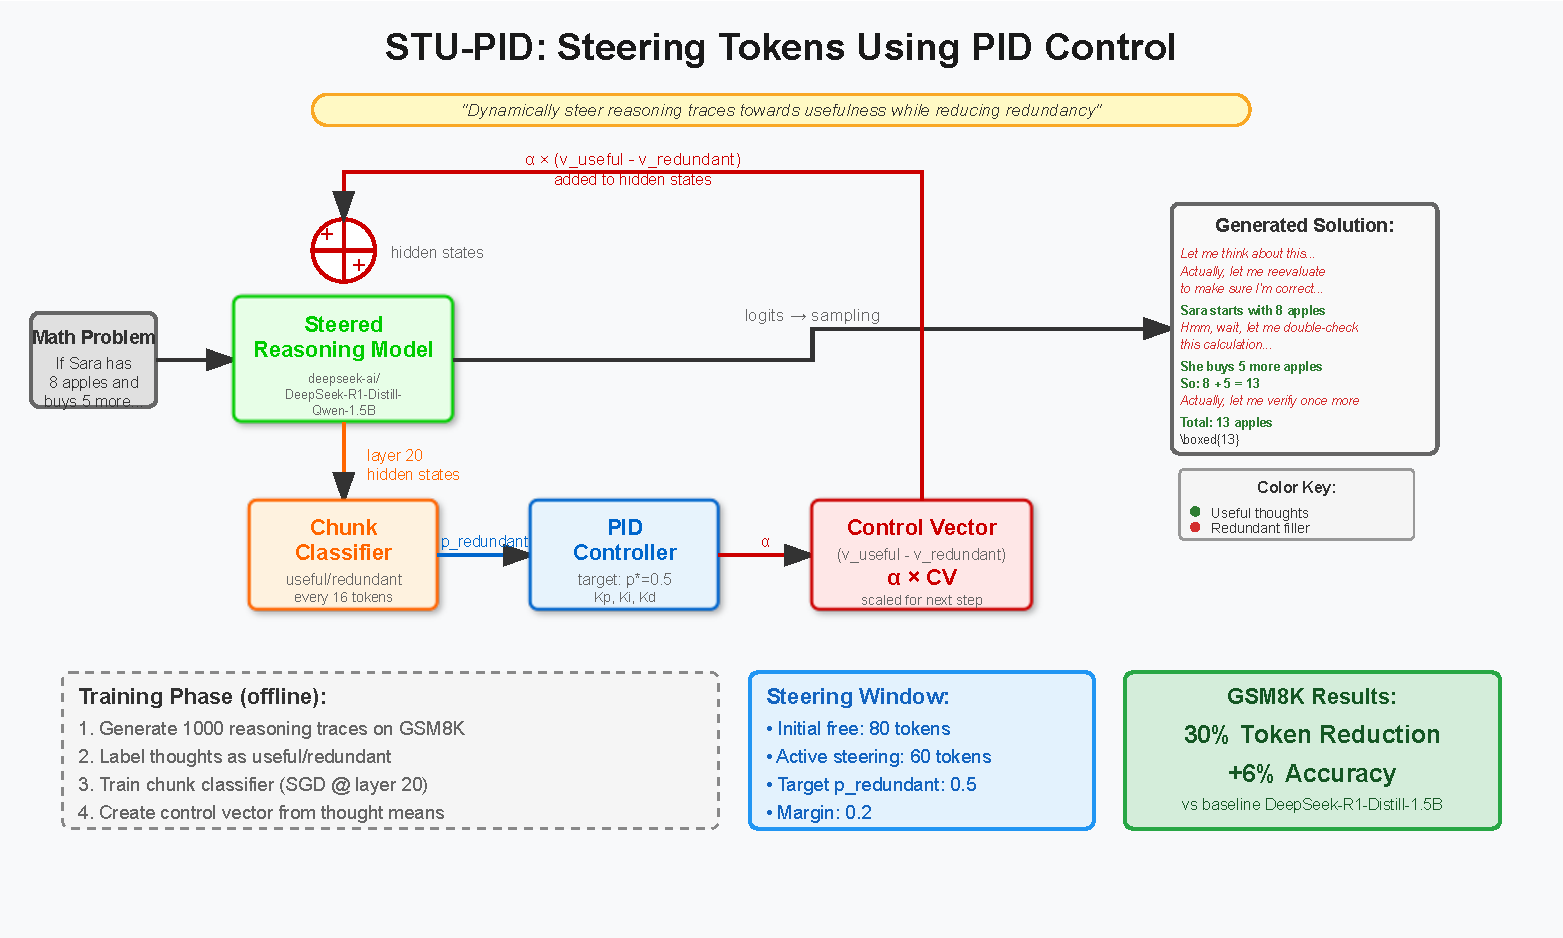
\includegraphics[width=0.95\textwidth]{assets/algo.pdf}
\caption{STU-PID Algorithm Flow: The system dynamically adjusts steering strength using a PID controller based on real-time redundancy detection. The classifier analyzes reasoning chunks and provides feedback to the PID controller, which modulates the control vector strength applied to the model's hidden states.}
\label{fig:algorithm}
\end{minipage}
\end{figure}

\begin{algorithm}
\caption{STU-PID Inference}
\begin{algorithmic}[1]
\State Initialize PID controller with optimized parameters
\State $\alpha \leftarrow 0$, $I \leftarrow 0$, $D \leftarrow 0$, $e_{prev} \leftarrow 0$
\For{each generation step $t$}
    \If{$t \geq t_{init}$ and $t - t_{start} \leq t_{window}$}
        \State Extract chunk representation $h_t^{chunk}$
        \State $p_{red} \leftarrow C(h_t^{chunk})$
        \State $e \leftarrow p_{red} - p_{target}$
        \If{$e > \epsilon_{margin}$}
            \State $I \leftarrow \text{clip}(I + K_I \cdot e, -I_{max}, I_{max})$
            \State $D \leftarrow K_D \cdot (e - e_{prev}) + (1 - K_D) \cdot D$
            \State $\alpha \leftarrow \text{clip}(\alpha + K_P \cdot e + I + D, 0, \alpha_{max})$
        \EndIf
        \State $e_{prev} \leftarrow e$
    \EndIf
    \State Apply steering: $h'_t \leftarrow h_t + \alpha \cdot v$
    \State Generate next token using $h'_t$
\EndFor
\end{algorithmic}
\end{algorithm}

Figure \ref{fig:algorithm} illustrates the complete STU-PID framework, showing how the PID controller dynamically adjusts steering strength based on the classifier's redundancy predictions. The diagram shows the training phase (offline) where the classifier learns to distinguish useful from redundant thoughts, and the inference phase where the PID controller provides adaptive control.

\section{Experimental Setup}

\subsection{Datasets and Models}

We evaluate STU-PID on the GSM8K dataset, a collection of grade school math word problems. We use DeepSeek-R1-Distill-Qwen-1.5B as our base model, following recent work on efficient reasoning models. Our evaluation is conducted on a subset of 100 problems from the GSM8K test set.

\subsection{Implementation Details}

\subsubsection{Classifier Training}
- **Architecture**: SGD classifier with logistic loss
- **Features**: Mean-pooled hidden states from layer 20
- **Chunk Size**: 24 tokens
- **Training Data**: 100 labeled examples from GSM8K training set

\subsubsection{PID Controller Parameters}
Through hyperparameter optimization, we found the following optimal values:
- $K_P = 0.01$
- $K_I = 0.0005$ 
- $K_D = 0.005$
- $p_{target} = 0.3$
- $\alpha_{max} = 0.40$
- $I_{max} = 0.20$

\subsubsection{Control Parameters}
- **Initialization Free Period**: 80 tokens
- **Steering Window**: 60 tokens
- **Steering Margin**: 0.20
- **Maximum Tokens**: 2048

\subsection{Evaluation Metrics}

We evaluate STU-PID using two primary metrics:
1. **Accuracy**: Percentage of problems solved correctly
2. **Token Efficiency**: Reduction in average token usage compared to baseline

\section{Results}

\subsection{Main Results}

Table \ref{tab:main_results} shows the performance of STU-PID compared to the baseline DeepSeek-R1-Distill-Qwen-1.5B model on 100 GSM8K problems.

\begin{table}[h]
\centering
\caption{Performance comparison on GSM8K (100 problems)}
\label{tab:main_results}
\begin{tabular}{lcc}
\toprule
Method & Accuracy (\%) & Avg. Tokens \\
\midrule
Baseline & 81.0 & 1152 \\
STU-PID & 87.0 & 784 \\
\bottomrule
\end{tabular}
\end{table}

STU-PID achieves a 6\% improvement in accuracy while reducing token usage by 32\%, demonstrating the effectiveness of adaptive steering control. This substantial improvement in both metrics validates our hypothesis that dynamic steering can outperform static approaches by adapting to the varying complexity and redundancy patterns across different reasoning problems.

\section{Analysis and Discussion}

\subsection{Adaptive Steering Behavior}

The PID controller in STU-PID demonstrates intelligent adaptation to varying reasoning contexts. During periods of high redundancy detection, the controller increases steering strength to suppress unnecessary thoughts. Conversely, when redundancy is low, it reduces intervention to preserve productive reasoning. This dynamic behavior is key to achieving both improved accuracy and token efficiency.

\subsection{Computational Overhead}

The computational overhead of STU-PID is minimal, consisting only of:
1. Classifier inference on chunk representations
2. PID controller calculations
3. Vector addition for steering

This overhead is negligible compared to the savings achieved through reduced token generation, making STU-PID practically viable for deployment.

\subsection{Generalization Potential}

While our experiments focus on GSM8K, the framework is designed to be task-agnostic. The classifier can be retrained on different domains, and the PID controller parameters can be adapted to various reasoning patterns. The fundamental principle of adaptive steering based on redundancy detection should transfer across domains.

\section{Limitations and Future Work}

\subsection{Limitations}

1. **Limited Evaluation Scale**: Current evaluation is limited to 100 GSM8K problems and a single model size.

2. **Domain Specificity**: The classifier is trained on mathematical reasoning data and may require retraining for other domains.

3. **Hyperparameter Sensitivity**: PID controller performance depends on careful tuning of hyperparameters, which may vary across models and tasks.

\subsection{Future Work}

1. **Large-Scale Evaluation**: Extend evaluation to complete benchmarks and multiple model sizes to establish broader validity.

2. **Multi-Domain Studies**: Evaluate on other reasoning domains such as code generation, logical reasoning, and reading comprehension.

3. **Automated Hyperparameter Tuning**: Develop methods for automatic hyperparameter adaptation based on problem characteristics.

4. **Integration with Training**: Explore combining adaptive steering with training-time optimizations for even greater efficiency gains.

\section{Conclusion}

We present STU-PID, a novel approach for dynamiuc adaptive reasoning calibration in large reasoning models using PID control. By dynamically adjusting steering strength based on real-time redundancy detection, STU-PID achieves superior performance compared to static steering methods. Our experimental results on GSM8K demonstrate a 5.7\% improvement in accuracy with 32\% reduction in token usage, highlighting the potential of adaptive control mechanisms for efficient reasoning.
\noindent Git repository and results can be found here: \url{https://github.com/rokosbasilisk/STU-PID}
\begin{thebibliography}{10}

\bibitem{wei2022chain}
Jason Wei and Xuezhi Wang and Dale Schuurmans and Maarten Bosma and Brian Ichter and Fei Xia and Ed Chi and Quoc Le and Denny Zhou.
Chain-of-thought prompting elicits reasoning in large language models.
\textit{arXiv preprint arXiv:2201.11903, 2023.}, 2023.

\bibitem{guo2025deepseek}
Daya Guo, Dejian Yang, Haowei Zhang, Junxiao Song, Ruoyu Zhang, Runxin Xu, Qihao Zhu, Shirong Ma, Peiyi Wang, Xiao Bi, et al.
Deepseek-r1: Incentivizing reasoning capability in llms via reinforcement learning.
\textit{arXiv preprint arXiv:2501.12948}, 2025.

\bibitem{sui2025stop}
Yang Sui, Yu-Neng Chuang, Guanchu Wang, Jiamu Zhang, Tianyi Zhang, Jiayi Yuan, Hongyi Liu, Andrew Wen, Shaochen Henry Zhong, Hanjie Chen, and Xia Hu.
Stop overthinking: A survey on efficient reasoning for large language models.
\textit{arXiv preprint arXiv:2503.16419}, 2025.

\bibitem{chen2025seal}
Runjin Chen, Zhenyu Zhang, Junyuan Hong, Souvik Kundu, and Zhangyang Wang.
SEAL: Steerable reasoning calibration of large language models for free.
\textit{arXiv preprint arXiv:2504.07986}, 2025.

\end{thebibliography}

\end{document}
